\chapter{Tokens become vectors}
\label{ch:emb}

\begin{question}
A model only takes numbers. Which numbers should stand for a token, so that similar words look similar to the model?
\end{question}

\begin{whatfor}
Token IDs are numbers, but the wrong kind. This chapter tries the simple fixes in turn (one-hot vectors, bag of words, n-grams) and shows where each fails. It then rebuilds word embeddings: dense vectors whose directions carry meaning, so that king $-$ man $+$ woman lands near queen. It shows how word2vec learns them (continuous bag of words and skip-gram), how an LLM keeps them in an embedding matrix that it trains with everything else, and how a positional vector tells the model where each token sits. The chapter's card is the input vector of a token.
\end{whatfor}

\begin{setup}
\textbf{The system:} the first layer of a GPT-style decoder.
\textbf{The one thing traced:} the token ``fox'' in ``The quick brown fox'', from token ID to the vector that enters the first block.
\end{setup}

\begin{recall}
\textbf{Recall.} A \emph{word embedding} gives each word a vector so that words used alike get similar vectors; the \emph{cosine similarity} $\cos(\mathbf u,\mathbf v) = \mathbf u\cdot\mathbf v / (\lVert\mathbf u\rVert\,\lVert\mathbf v\rVert)$ measures how alike two vectors point. Chapter 9: a \emph{token ID} is a token's number in the vocabulary.
\end{recall}

%=====================================================================
\section{Words you need}

\subsection*{Why token IDs are not enough}

\begin{definition}[Ordinal number problem]
A model treats inputs as quantities: 21 is close to 22 and far from 6. That fits ordinal data, where the order means something (low $<$ medium $<$ high). Token IDs are only labels, so feeding them in as quantities invents closeness that isn't there: the \dfn{ordinal number problem}.
\end{definition}

\begin{example}[Good, great, bad]
Suppose good $= 6$, great $= 21$, bad $= 22$.
\begin{steps}
  \item Distance great to bad: $|22 - 21| = 1$.
  \item Distance great to good: $|21 - 6| = 15$.
  \item So ``great'' looks 15 times closer to ``bad'' than to ``good'', the opposite of their meaning. A sentiment model fed these IDs is misled from the start.
\end{steps}
\end{example}

\begin{definition}[One-hot vector]
A \dfn{one-hot vector} for a token is a vector as long as the vocabulary, with a 1 in that token's position and 0 everywhere else. Every pair of different words is then equally far apart, so no false order is invented.
\end{definition}

\begin{example}[One-hot, vocabulary of six]
Vocabulary: This, movie, was, good, bad, great.
\begin{steps}
  \item This $= (1,0,0,0,0,0)$, movie $= (0,1,0,0,0,0)$, \dots, great $= (0,0,0,0,0,1)$.
  \item ``This movie was good'' is four vectors: $(1,0,0,0,0,0)$, $(0,1,0,0,0,0)$, $(0,0,1,0,0,0)$, $(0,0,0,1,0,0)$.
  \item ``good'' and ``great'' share no 1: one-hot sees them as no more alike than ``good'' and ``movie''.
\end{steps}
\end{example}

\begin{result}[What one-hot costs]
Simple, and no false order. But:
\begin{itemize}
  \item \textbf{Sparse and large:} with GPT-2's 50,257 tokens, every token is 50,257 numbers, all but one zero. Memory and computation are wasted.
  \item \textbf{No meaning:} every word is equally unlike every other, so ``good'' and ``great'' look unrelated.
\end{itemize}
\end{result}

\begin{definition}[Bag of words, n-gram]
A \dfn{bag of words} turns a whole sentence into one vector: count how often each vocabulary word appears, ignoring order. Counting single words is the unigram version. An \dfn{n-gram} is a run of $n$ consecutive words; counting bigrams ($n=2$), trigrams ($n=3$) and so on adds a little local order.
\end{definition}

\begin{example}[Unigram and bigram counts]
Sentences: (1) ``This movie was good'', (2) ``This movie was bad''.
\begin{steps}
  \item Unigram columns This, movie, was, good, bad: (1) $= (1,1,1,1,0)$, (2) $= (1,1,1,0,1)$.
  \item Bigram columns ``This movie'', ``movie was'', ``was good'', ``was bad'': (1) $= (1,1,1,0)$, (2) $= (1,1,0,1)$.
\end{steps}
\end{example}

\begin{result}[Where n-grams stop]
The number of possible n-grams explodes with the data, so the vectors are huge and sparse. Context reaches only $n$ words. And they still carry no word meaning, which translation and text generation need.
\end{result}

\subsection*{Two kinds of meaning}

\begin{definition}[Semantic and contextual meaning]
\dfn{Semantic meaning} is what a word means on its own: swap a word for a synonym and the sentence still says the same thing. \dfn{Contextual meaning} is what a word means in this sentence: which word it describes, what it refers back to.
\end{definition}

\begin{example}[Predicting after ``the dusty'']
``Mia walked into the old museum. Her hands were shaking. She knew something was hidden behind the dusty \dots''
\begin{steps}
  \item Contextual: ``old'' describes the museum, not Mia; Mia is going into the museum.
  \item Semantic: things in an old museum that can be dusty, such as a cabinet, a curtain or a painting.
  \item So the likely next words are ``cabinet'', ``curtain'', ``painting''. Embeddings supply the semantic part; attention, in the next chapter, the contextual part.
\end{steps}
\end{example}

\subsection*{Word embeddings}

\begin{definition}[Embedding space]
A word embedding is a dense vector: every entry is used, and a few hundred or a few thousand entries are enough, against hundreds of thousands for one-hot. The vectors live in the \dfn{embedding space}, where closeness means similar words and directions carry meaning. Which feature each direction holds is not chosen: it comes out of training, starting from random vectors.
\end{definition}

\begin{example}[Features you could imagine]
In one dimension, put people on an age line: people of similar age sit close together. In two dimensions, use age and royalty: king and queen sit together, high on royalty, and away from man and woman. Real embeddings learn their own dimensions, but the picture is the same.
\end{example}

\begin{definition}[Vector analogy]
Because directions carry meaning, a difference of two embeddings is itself meaningful. A \dfn{vector analogy}: king $-$ man $+$ woman $\approx$ queen, because ``king minus man'' is roughly the royalty direction. Another: Beijing $-$ China $+$ Japan $\approx$ Tokyo, since taking away China and adding Japan leaves ``capital city of Japan''.
\end{definition}

\begin{example}[King $-$ man $+$ woman, in five features]
Features: masculine, wealth, power, weight, speech.
king $(0.9, 0.8, 0.9, 0.7, 0.6)$, man $(0.9, 0.2, 0.3, 0.7, 0.6)$, woman $(0.1, 0.2, 0.3, 0.5, 0.6)$, queen $(0.1, 0.8, 0.8, 0.5, 0.6)$, cat $(0.5, 0.0, 0.0, 0.1, 0.0)$.
\begin{steps}
  \item Result $r$ = king $-$ man $+$ woman $= (0.1, 0.8, 0.9, 0.5, 0.6)$.
  \item Lengths: $\lVert r\rVert = \sqrt{2.07} = 1.439$, $\lVert\text{queen}\rVert = \sqrt{1.90} = 1.378$, $\lVert\text{cat}\rVert = \sqrt{0.26} = 0.510$.
  \item With queen: $r\cdot\text{queen} = 1.98$, so $\cos = 1.98/(1.439 \times 1.378) = 0.998$.
  \item With cat: $r\cdot\text{cat} = 0.10$, so $\cos = 0.10/(1.439 \times 0.510) = 0.136$.
  \item $r$ points almost exactly the way queen does, and nowhere near cat.
\end{steps}
\end{example}

\begin{remark}[Seeing the space]
Embeddings with hundreds of dimensions can't be drawn, but principal component analysis (PCA) projects them to two or three. In a trained model the picture shows clusters: words about tennis together, words about cats together, the digit ``one'' with ``1'' and its relatives.
\end{remark}

\subsection*{Learning embeddings: word2vec}

\begin{definition}[Continuous bag of words]
\dfn{Word2vec} learns embeddings with a small neural network. Its first method, \dfn{continuous bag of words} (CBOW), slides a window over the text; the middle word is the target and its neighbours are the context. With a window of 3 (one word each side), ``fox \_\_ over'' must predict ``jumps''.
\begin{itemize}
  \item Input layer: the one-hot vectors of the context words, $V$ numbers each.
  \item Hidden layer: $d$ neurons, $d$ being the embedding size wanted (3 in the toy, hundreds in practice).
  \item Last layer: $V$ neurons, one per vocabulary word, softmax-ed into probabilities for the target.
\end{itemize}
The error against the true target is back-propagated, the weights adjusted, and the window moves on.
\end{definition}

\begin{definition}[Skip-gram]
\dfn{Skip-gram} is CBOW reversed: the middle word is the input and the model predicts each neighbour. From ``jumps'' it must predict ``fox'' and ``over''. Both methods learn good embeddings.
\end{definition}

\begin{definition}[Embedding matrix]
After training, the input-to-hidden weights form the \dfn{embedding matrix} $E$, with $V$ rows (one per vocabulary word) and $d$ columns (the embedding size). Row $i$ is word $i$'s embedding, so $E$ is a lookup table. Multiplying a one-hot row vector by $E$ picks out that row.
\end{definition}

\begin{example}[Looking up ``fox'']
Vocabulary of 8: the, quick, brown, fox, jumps, over, lazy, dog. Embedding size 3, so $E$ is $8 \times 3$; its fourth row is fox $= (0.7, -0.1, 0.4)$.
\begin{steps}
  \item One-hot for fox: $o = (0,0,0,1,0,0,0,0)$.
  \item $oE$ = $0\cdot\text{row}_1 + 0\cdot\text{row}_2 + 0\cdot\text{row}_3 + 1\cdot\text{row}_4 + 0 + \dots = \text{row}_4 = (0.7, -0.1, 0.4)$.
  \item In practice nothing is multiplied: the token ID 4 indexes row 4 directly.
\end{steps}
\end{example}

\subsection*{Embeddings inside an LLM}

\begin{remark}[The embedding layer]
An LLM does not use word2vec. Its first layer is an embedding layer: an embedding matrix $E$ of size $V \times d$ whose entries are weights, trained together with the whole model by the next-token loss. For $n$ input tokens it returns an $n \times d$ matrix, one row per token.
\end{remark}

\begin{definition}[Output layer]
The \dfn{output layer} is the last layer: a linear layer from $d$ numbers to $V$ numbers, the logits of chapter 8, one per vocabulary token. It is the embedding layer's mirror image: $d \to V$ instead of $V \to d$.
\end{definition}

\begin{definition}[Positional vector]
An RNN reads tokens one after another, so it knows their order. A Transformer reads them all in parallel and doesn't. So a \dfn{positional vector} $p_t$, one per position $t$, is added to each token's embedding. It can be learned (a trainable table, one row per position) or a fixed pattern of numbers unique to each position. Adding it keeps the shape, $n \times d$; only the values shift.
\end{definition}

\begin{example}[``fox'' at position 4]
In ``The quick brown fox'', fox sits at position 4. Suppose $p_4 = (0.1, 0.0, -0.2)$.
\begin{steps}
  \item Embedding row: $(0.7, -0.1, 0.4)$.
  \item Add the position: $(0.7 + 0.1,\ -0.1 + 0.0,\ 0.4 - 0.2) = (0.8, -0.1, 0.2)$.
  \item This vector, meaning plus position, is what enters the first block of the decoder.
\end{steps}
\end{example}

\begin{sayit}[Say it in 20 seconds]
Token IDs can't go in raw: the model would read 21 as close to 22. One-hot fixes that but is huge, sparse and meaningless; n-grams add local order but explode in size. Embeddings are dense vectors where similar words sit close and directions carry meaning; word2vec learns them by predicting a word from its neighbours. In an LLM the embedding matrix is just the first layer, trained with everything else, and a positional vector is added so the model knows the order.
\end{sayit}

%=====================================================================
\section{The picture}

\begin{sayit}[Board 10.1 · IDs as numbers invent closeness]
\begin{pic}
\begin{tikzpicture}[font=\sffamily\small,x=0.55cm]
\draw[->,prec] (0,0) -- (24,0);
\foreach \x in {0,5,10,15,20} \draw[prec] (\x,0.1) -- (\x,-0.1) node[below,font=\sffamily\scriptsize] {\x};
\foreach \x/\w/\c/\a in {6/good/thmc/south,21/great/thmc/south east,22/bad/trapc/south west} {\fill[\c] (\x,0) circle (2.5pt); \node[anchor=\a,text=\c] at (\x,0.1) {\w};}
\draw[<->,trapc] (21,-0.7) -- node[below,font=\sffamily\scriptsize] {1} (22,-0.7);
\draw[<->,thmc] (6,-0.7) -- node[below,font=\sffamily\scriptsize] {15} (21,-0.7);
\end{tikzpicture}
\end{pic}
Say: ``IDs are labels, not quantities. Read as numbers, great is next to bad and far from good.''
\end{sayit}

\begin{sayit}[Board 10.2 · One-hot: equal and empty]
\begin{pic}
\begin{tikzpicture}[font=\sffamily\scriptsize]
\foreach \w [count=\i from 0] in {This,movie,was,good,bad,great} {
  \node[anchor=east] at (-0.1,-\i*0.42) {\w};
  \node[rotate=60,anchor=west] at (\i*0.5,0.3) {\w};
  \foreach \j in {0,...,5} {\pgfmathsetmacro{\v}{\i==\j ? 1 : 0}
    \ifnum\i=\j \fill[thmc!40] (\j*0.5-0.25,-\i*0.42-0.21) rectangle (\j*0.5+0.25,-\i*0.42+0.21);\fi
    \node at (\j*0.5,-\i*0.42) {\pgfmathprintnumber[int detect]{\v}};}}
\node[anchor=west,font=\sffamily\small,align=left] at (3.6,-1.0) {GPT-2: 50,257 entries per token,\\one of them 1, the rest 0};
\end{tikzpicture}
\end{pic}
Say: ``One-hot removes the false order: every word is equally far from every other. But that means good and great are as unrelated as good and movie, and each vector is as long as the vocabulary.''
\end{sayit}

\begin{sayit}[Board 10.3 · Bag of words and bigrams]
\begin{pic}
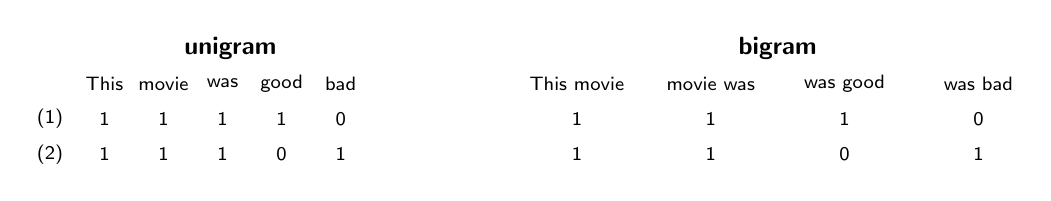
\begin{tikzpicture}[font=\sffamily\scriptsize]
\node[font=\sffamily\small\bfseries] at (1.6,0.9) {unigram};
\foreach \h [count=\j from 0] in {This,movie,was,good,bad} \node at (\j*0.75,0.45) {\h};
\foreach \r/\vals [count=\i from 0] in {(1)/{1,1,1,1,0},(2)/{1,1,1,0,1}} {
  \node[anchor=east] at (-0.4,-\i*0.45) {\r};
  \foreach \v [count=\j from 0] in \vals \node at (\j*0.75,-\i*0.45) {\v};}
\node[font=\sffamily\small\bfseries] at (8.55,0.9) {bigram};
\foreach \h [count=\j from 0] in {This movie,movie was,was good,was bad} \node at (6.0+\j*1.7,0.45) {\h};
\foreach \vals [count=\i from 0] in {{1,1,1,0},{1,1,0,1}} {
  \foreach \v [count=\j from 0] in \vals \node at (6.0+\j*1.7,-\i*0.45) {\v};}
\end{tikzpicture}
\end{pic}
Say: ``Count the words, or count the word pairs. Pairs keep a little order, but the number of possible pairs, triples and so on blows up.''
\end{sayit}

\begin{sayit}[Board 10.4 · Semantic against contextual]
\begin{pic}
\begin{tikzpicture}[>={Latex[length=2mm]},font=\sffamily\small]
\node[anchor=west] (s) at (0,0) {Mia walked into the \textbf{old} \textbf{museum}. \dots\ hidden behind the \textbf{dusty} \_\_\_};
\draw[->,thmc,thick] (4.35,0.25) to[bend left=50] node[above,font=\sffamily\scriptsize]{describes} (5.25,0.25);
\draw[->,defc,thick] (11.2,-0.25) to[bend left=25] node[below,font=\sffamily\scriptsize]{what can be dusty in a museum?} (5.3,-0.25);
\node[anchor=west,font=\sffamily\scriptsize,text=prec] at (0,-2.0) {semantic: what each word means $\cdot$ contextual: how the words connect here};
\end{tikzpicture}
\end{pic}
Say: ``To guess the next word you need both: what words mean, and which words go with which in this sentence. Embeddings give the first; attention gives the second.''
\end{sayit}

\begin{sayit}[Board 10.5 · An embedding space you can draw]
\begin{pic}
\begin{tikzpicture}[>={Latex[length=2mm]},font=\sffamily\small]
\draw[->,prec] (0,0) -- (6.5,0) node[below left,font=\sffamily\scriptsize] {age};
\draw[->,prec] (0,0) -- (0,4.2) node[above,font=\sffamily\scriptsize] {royalty};
\foreach \x/\y/\w in {1.2/0.8/boy,1.4/0.6/girl,4.2/0.9/man,4.6/0.5/woman,4.4/3.5/king,4.9/3.3/queen,1.3/3.0/prince} {\fill[defc] (\x,\y) circle (2pt); \node[anchor=south west,font=\sffamily\scriptsize] at (\x,\y) {\w};}
\draw[->,thmc,thick] (4.2,0.9) -- (4.4,3.5); \draw[->,thmc,thick] (4.6,0.5) -- (4.9,3.3);
\node[font=\sffamily\scriptsize,text=thmc,anchor=west] at (5.2,2.1) {same direction:};
\node[font=\sffamily\scriptsize,text=thmc,anchor=west] at (5.2,1.7) {``add royalty''};
\end{tikzpicture}
\end{pic}
Say: ``Similar words sit close; the arrow from man to king is the same as from woman to queen. That's why king minus man plus woman lands on queen.''
\end{sayit}

\begin{sayit}[Board 10.6 · The analogy in five features]
\begin{pic}
\begin{tikzpicture}[font=\sffamily\scriptsize]
\foreach \f [count=\j from 0] in {masc.,wealth,power,weight,speech} \node at (2+\j*1.1,0.5) {\f};
\foreach \w/\vals/\c [count=\i from 0] in {king/{0.9,0.8,0.9,0.7,0.6}/bdq,$-$ man/{0.9,0.2,0.3,0.7,0.6}/bdq,$+$ woman/{0.1,0.2,0.3,0.5,0.6}/bdq,$= r$/{0.1,0.8,0.9,0.5,0.6}/bdy,queen/{0.1,0.8,0.8,0.5,0.6}/bdg,cat/{0.5,0.0,0.0,0.1,0.0}/bdr} {
  \node[anchor=east] at (1.3,-\i*0.5) {\w};
  \foreach \v [count=\j from 0] in \vals {\fill[\c,draw=\c L] (1.6+\j*1.1,-\i*0.5-0.2) rectangle (2.4+\j*1.1,-\i*0.5+0.2); \node at (2+\j*1.1,-\i*0.5) {\v};}}
\node[anchor=west] at (7.3,-2.0) {$\cos(r,\text{queen}) = 0.998$};
\node[anchor=west] at (7.3,-2.5) {$\cos(r,\text{cat}) = 0.136$};
\end{tikzpicture}
\end{pic}
Say: ``Subtract man, add woman: only the masculine and weight entries change, and the result is almost exactly queen.''
\end{sayit}

\begin{sayit}[Board 10.7 · Clusters after training (2-D projection)]
\begin{pic}
\begin{tikzpicture}[font=\sffamily\scriptsize]
\draw[prec!50] (-3.5,0) -- (3.5,0); \draw[prec!50] (0,-1.8) -- (0,1.8);
\foreach \x/\y/\w in {-2.8/1.4/banana,-3.2/0.9/orange,-2.1/0.6/apple} {\fill[exc] (\x,\y) circle (2pt); \node[anchor=west] at (\x,\y) {\w};}
\foreach \x/\y/\w in {1.6/1.4/king,2.6/1.2/man,2.0/0.7/woman} {\fill[defc] (\x,\y) circle (2pt); \node[anchor=west] at (\x,\y) {\w};}
\foreach \x/\y/\w in {-2.6/-0.7/tennis,-3.2/-1.2/golf,-2.0/-1.5/hockey} {\fill[thmc] (\x,\y) circle (2pt); \node[anchor=west] at (\x,\y) {\w};}
\foreach \x/\y/\w in {1.9/-0.8/dog,2.4/-1.1/cat,2.1/-1.5/cow} {\fill[trapc] (\x,\y) circle (2pt); \node[anchor=west] at (\x,\y) {\w};}
\end{tikzpicture}
\end{pic}
Say: ``Projected down with PCA, trained embeddings fall into clusters by topic: fruit, people, sports, animals. Nobody labelled those groups; training found them.''
\end{sayit}

\begin{sayit}[Board 10.8 · CBOW and skip-gram windows]
\begin{pic}
\begin{tikzpicture}[>={Latex[length=2mm]},font=\sffamily\small,
  w/.style={draw=#1L,fill=#1,rounded corners=1pt,inner sep=3pt,minimum height=6mm}]
\foreach \t/\c [count=\i from 0] in {The/bdq,quick/bdq,brown/bdq,fox/bdv,jumps/bdg,over/bdv,the/bdq,lazy/bdq,dog/bdq} \node[w=\c] (t\i) at (\i*1.35,0) {\t};
\node[font=\sffamily\small\bfseries,anchor=east] at (-0.6,-1.2) {CBOW};
\node[w=bdv] (c1) at (2.0,-1.2) {fox}; \node[w=bdv] (c2) at (3.4,-1.2) {over}; \node[w=bdg] (c3) at (6.2,-1.2) {jumps};
\draw[->] (3.95,-1.2) -- (c3);
\node[font=\sffamily\small\bfseries,anchor=east] at (-0.6,-2.2) {skip-gram};
\node[w=bdg] (s1) at (2.7,-2.2) {jumps}; \node[w=bdv] (s2) at (6.0,-2.0) {fox}; \node[w=bdv] (s3) at (6.0,-2.6) {over};
\draw[->] (s1) -- (s2.west); \draw[->] (s1) -- (s3.west);
\node[font=\sffamily\scriptsize,text=prec,anchor=west] at (7.5,-1.7) {then slide the window one word};
\end{tikzpicture}
\end{pic}
Say: ``CBOW predicts the middle word from its neighbours; skip-gram predicts the neighbours from the middle word. Either way, words that share neighbours end up with similar vectors.''
\end{sayit}

\begin{sayit}[Board 10.9 · The CBOW network]
\begin{pic}
\begin{tikzpicture}[font=\sffamily\scriptsize]
\foreach \i in {1,...,8} {\node[draw=bdqL,fill=bdq,circle,inner sep=1.5pt] (a\i) at (0,-\i*0.42) {}; \node[draw=bdgL,fill=bdg,circle,inner sep=1.5pt] (c\i) at (5,-\i*0.42) {};}
\foreach \j in {1,2,3} \node[draw=bdvL,fill=bdv,circle,inner sep=2.5pt] (b\j) at (2.5,-0.84-\j*0.42) {};
\foreach \i in {1,...,8} \foreach \j in {1,2,3} {\draw[prec!50] (a\i) -- (b\j); \draw[prec!50] (b\j) -- (c\i);}
\node[align=center] at (0,0.2) {input: one-hot\\$V = 8$};
\node[align=center] at (2.5,0.2) {hidden\\$d = 3$};
\node[align=center] at (5,0.2) {output: softmax\\$V = 8$};
\node[draw=defc,rounded corners=2pt,align=center] at (1.25,-4.1) {these weights $= E$ ($8 \times 3$)};
\node[anchor=west,align=left] at (5.6,-1.9) {target: ``jumps''\\error $\to$ back-propagate};
\end{tikzpicture}
\end{pic}
Say: ``A one-layer network. The weights into the hidden layer, eight rows of three, are the embeddings: that's the product, the prediction task is only the excuse.''
\end{sayit}

\begin{sayit}[Board 10.10 · One-hot times $E$ picks a row]
\begin{pic}
\begin{tikzpicture}[font=\sffamily\scriptsize]
\node[draw=bdqL,fill=bdq,inner sep=3pt] (o) at (0,0) {$(0,0,0,1,0,0,0,0)$};
\node at (1.8,0) {$\times$};
\foreach \w/\r [count=\i from 0] in {the/{0.1, 0.3, -0.2},quick/{0.5, -0.4, 0.2},brown/{0.2, 0.1, 0.6},fox/{0.7, -0.1, 0.4},jumps/{-0.3, 0.8, 0.1},over/{0.0, 0.2, -0.5},lazy/{0.4, 0.4, 0.3},dog/{0.6, 0.0, 0.5}} {
  \ifnum\i=3 \fill[thmc!30] (2.3,1.5-\i*0.4) rectangle (5.0,1.9-\i*0.4);\fi
  \node[anchor=east] at (2.3,1.7-\i*0.4) {\w};
  \node at (3.65,1.7-\i*0.4) {$(\r)$};}
\draw[defc] (2.3,-1.7) rectangle (5.0,1.9);
\node at (5.5,0) {$=$};
\node[draw=bdgL,fill=bdg,inner sep=3pt] at (7.1,0) {$(0.7, -0.1, 0.4)$};
\end{tikzpicture}
\end{pic}
Say: ``Multiplying a one-hot vector by the embedding matrix just picks out one row, so in practice the token ID is used as a row index.''
\end{sayit}

\begin{sayit}[Board 10.11 · Embeddings inside the decoder]
\begin{pic}
\begin{tikzpicture}[>={Latex[length=2mm]},font=\sffamily\small,
  box/.style={draw=#1L,fill=#1,rounded corners=2pt,align=center,minimum height=10mm,inner sep=3pt,text width=21mm}]
\node[box=bdq] (a) at (0,0) {The quick brown fox};
\node[box=bdq] (b) at (2.75,0) {IDs\\1, 2, 3, 4};
\node[box=bdv] (c) at (5.5,0) {embedding\\$E$: $V \times d$};
\node[box=bdy] (d) at (8.25,0) {$+$ positional\\vectors};
\node[box=bda] (e) at (11.0,0) {decoder blocks};
\node[box=bdg] (f) at (11.0,-1.9) {output layer\\$d \to V$ logits};
\node[font=\sffamily\scriptsize,text=prec] at (6.9,-1.1) {each arrow after $E$ carries a $4 \times d$ matrix};
\draw[->] (a) -- (b); \draw[->] (b) -- (c); \draw[->] (c) -- (d); \draw[->] (d) -- (e); \draw[->] (e) -- (f);
\end{tikzpicture}
\end{pic}
Say: ``IDs index rows of the embedding matrix, positions are added, the blocks work on an $n \times d$ matrix, and the output layer maps back from $d$ to the whole vocabulary.''
\end{sayit}

%=====================================================================
\section{How it works}
\begin{enumerate}
  \item Each token ID picks its row of the embedding matrix $E$ ($V \times d$): $n$ tokens give an $n \times d$ matrix.
  \item The positional vector for each position is added; the shape stays $n \times d$.
  \item The blocks of the decoder turn these meaning-plus-position vectors into context-aware ones (next chapter).
  \item The output layer maps each final vector from $d$ numbers to $V$ logits.
  \item The next-token loss trains $E$, the positional table (if learned) and everything else together.
\end{enumerate}

%=====================================================================
\section*{Formula sheet}
\addcontentsline{toc}{section}{Formula sheet}

\begin{mastercard}[label=card:input]{Input vector of a token}
A token enters the model as its embedding row plus the vector for its position. With $E$ the $V \times d$ embedding matrix, $o_t$ the one-hot row vector of the token at position $t$ (length $V$), $\mathrm{id}_t$ its token ID and $p_t$ the positional vector (length $d$):
\[
\boxed{x_t = o_t\,E + p_t = E[\mathrm{id}_t] + p_t, \qquad X = O\,E + P \ \ (n \times d).}
\]
\begin{plugrows}
  \plugrow{Embedding look-up only (word2vec, or before positions)}{\pstep{Box: $x_t = o_t E + p_t$.}\pstep{No position added: $p_t = 0$.}\pstep{$o_t$ has a single 1 at $\mathrm{id}_t$, so $o_t E$ is row $\mathrm{id}_t$ of $E$.}}{$x_t = E[\mathrm{id}_t]$}{any embedding table}{8 words, $d = 3$, fox $=$ ID 4: $(0,0,0,1,0,0,0,0)\,E = \text{row}_4 = (0.7, -0.1, 0.4)$}
  \plugrow{A token at a position (LLM input)}{\pstep{Box: $x_t = E[\mathrm{id}_t] + p_t$.}\pstep{Row from $E$: the token's embedding.}\pstep{$p_t$ from the positional table at position $t$.}\pstep{Add entry by entry.}}{$x_t$, length $d$}{Transformer input}{fox at $t = 4$, $p_4 = (0.1, 0.0, -0.2)$: $(0.7 + 0.1, -0.1 + 0, 0.4 - 0.2) = (0.8, -0.1, 0.2)$}
  \plugrow{A whole sequence}{\pstep{Box: $X = OE + P$.}\pstep{$O$: $n$ one-hot rows, so $n \times V$; $E$: $V \times d$; $P$: the first $n$ positional rows, $n \times d$.}\pstep{Shapes: $(n \times V)(V \times d) = n \times d$, and adding $P$ keeps $n \times d$.}}{$X$ is $n \times d$}{$n \le$ context window}{6 tokens, $d = 768$: $X$ is $6 \times 768 = 4{,}608$ numbers}
  \plugrow{One-hot input, no learned embedding}{\pstep{Box: $x_t = o_t E + p_t$.}\pstep{No embedding: $E = I$, the $V \times V$ identity, so $d = V$; no position: $p_t = 0$.}\pstep{$o_t I = o_t$.}}{$x_t = o_t$, length $V$}{bag-of-words style models}{GPT-2: $V = 50{,}257$ numbers per token against $d = 768$: $50{,}257/768 = 65.4$ times longer}
\end{plugrows}
\end{mastercard}

\begin{intuition}
An embedding is a learned coordinate system for meaning. Training never says ``this axis is royalty''; it only rewards vectors that help predict neighbours (word2vec) or the next token (an LLM), and similar words end up close because they predict the same things.
\end{intuition}

%=====================================================================
\section{What they will ask}

\begin{iq}[\core]{Why not feed token IDs straight into the model?}
The model would read them as quantities: with good 6, great 21, bad 22, great looks 15 times closer to bad than to good. IDs are labels, so they need a representation without a false order.
\end{iq}

\begin{iq}[\core]{One-hot against embeddings?}
One-hot: length $V$ (50,257 for GPT-2), one 1, no false order but no meaning either: every word is equally unlike every other. Embeddings: dense, a few hundred numbers, learned so that similar words are close and directions mean something.
\end{iq}

\begin{iq}[\core]{How does word2vec learn embeddings?}
A small network predicts a word from its context (CBOW) or the context from a word (skip-gram), sliding a window over text. The input-to-hidden weights, $V \times d$, are kept as the embedding matrix.
\end{iq}

\begin{iq}[\core]{How are embeddings done in an LLM?}
An embedding layer: a $V \times d$ matrix of trainable weights, indexed by token ID, trained with the whole model on next-token prediction. A positional vector is added to each row. The output layer at the end maps $d$ back to $V$ logits.
\end{iq}

\begin{iq}[\core]{Why add a positional vector?}
Attention reads all tokens in parallel and has no built-in order, unlike an RNN. Adding a position vector, learned or fixed, to each embedding tells the model where each token is, without changing the $n \times d$ shape.
\end{iq}

\begin{iq}{Explain king $-$ man $+$ woman $\approx$ queen.}
Directions in embedding space carry meaning: king $-$ man is roughly ``royalty''. Adding it to woman lands near queen. With five toy features the result has cosine 0.998 with queen and 0.136 with cat.
\end{iq}

\begin{iq}{What does the embedding not give you?}
Context. ``Bank'' gets one vector whatever the sentence. Working out which word ``old'' describes, or what ``it'' refers to, is attention's job.
\end{iq}

\begin{iq}{Bag of words and n-grams: why not enough?}
They count words or short runs of words. The vectors become huge and sparse as $n$ grows, context reaches only $n$ words, and there's still no notion that two words mean similar things.
\end{iq}
